\chapter{Introduction}

You discover a new protein sequence family, and carefully construct a
multiple sequence alignment. Your family, like most protein families,
has a number of strongly (but not absolutely) conserved key residues,
separated by characteristic spacing. You wonder if there are more
members of your family in the sequence databases, but the family is so
evolutionarily diverse, a BLAST search with any individual sequence
doesn't even find the rest of the sequences you already know about;
you're sure there are some distantly related sequences in the
``noise''. You spend many pleasant evenings scanning weak BLAST
alignments by eye to find ones with the right key residues are in the
right places. You sure wish there was a computer program that did this
better.

You get the sequence of another favorite protein and eagerly BLAST it
against the NCBI server, and nothing significant shows up. It looks
like you'll get no easy information from the sequence.

You BLAST another favorite sequence against the NCBI server; a
thousand hits come back, and the top hundred are hypothetical
sequences from genome projects. It looks like you'll have to wade
through a lot of BLAST output to find the informative hits.

Another sequence comes back a slew of hits to receptor tyrosine
kinases, but before you decide to call your sequence an RTK homologue,
you recall that RTK's are, like many proteins, composed of multiple
functional domains. Is your sequence really an RTK? Or is it a novel
sequence that also happens to have a protein kinase catalytic domain,
fibronectin type III domain, or immunoglobulin superfamily domain?

These (and other problems in sequence analysis) are the kinds of
problems that HMMER tries to address. 

\section {Profile HMMs}

Profile hidden Markov models (profile HMMs) are statistical models of
the primary structure consensus of a sequence family. Anders Krogh,
David Haussler, and co-workers at UC Santa Cruz introduced profile
HMMs \cite{Krogh94}, adopting HMM techniques which have been used for
years in speech recognition. HMMs had been used in biology before the
Krogh/Haussler work, but the Krogh paper had a particularly dramatic
impact, because HMM technology was so well-suited to the popular
``profile'' methods for searching databases using multiple sequence
alignments instead of single query sequences. Since then, several
computational biology groups (including ours) have rapidly adopted
HMMs as the underlying formalism for sequence profile analysis.

``Profiles'' were introduced by Gribskov and colleagues
\cite{Gribskov87,Gribskov90} at about the same time
that other groups introduced similar approaches, such as ``flexible
patterns'' \cite{Barton90}, and
``templates''\cite{Bashford87,Taylor86}. The term ``profile'' has
stuck.\footnote{There has been some agitation to call all such models
``position specific scoring matrices'', PSSMs, but certain small
nocturnal North American marsupials have a prior claim on the
mnemonic.}  All of these are more or less statistical descriptions of
the consensus of a multiple sequence alignment. They use
position-specific scores for amino acids (or nucleotides) and position
specific scores for opening and extending an insertion or deletion.
Traditional pairwise alignment (for example, BLAST
\cite{Altschul90}, FASTA \cite{Pearson88}, or the Smith/Waterman
algorithm \cite{Smith81}) uses position-{\em independent} scoring
parameters. This property of profiles captures important information
about the degree of conservation at various positions in the multiple
alignment, and the varying degree to which gaps and insertions are
permitted.

The advantage of using HMMs is that HMMs have a formal probabilistic
basis. We can use Bayesian probability theory to guide how all the
probability (scoring) parameters should be set. Though this might
sound like a purely academic issue, this probabilistic basis lets us
do things that the more heuristic methods cannot do easily. For
example, an HMM can be trained from unaligned sequences, if a trusted
alignment isn't yet known. Another consequence is that HMMs have a
consistent theory behind gap and insertion scores.\footnote{
Surprisingly, this is still controversial.  People have been saying
``there is no theory for setting gap scores'' for so long that many
people believe it.} In most details, HMMs are a slight improvement
over a carefully constructed profile -- but far less skill and manual
intervention is necessary to train a good HMM and use it.  This allows
us to make libraries of hundreds of profile HMMs and apply them on a
very large scale to whole-genome or EST sequence analysis.  One such
database of protein domain models is Pfam \cite{Sonnhammer97}; the
construction and use of Pfam is tightly tied to the HMMER software
package.

HMMs do have important limitations. One is that HMMs do not capture
any higher-order correlations.  An HMM assumes that the identity of a
particular position is independent of the identity of all other
positions.\footnote{This is not strictly true. There is a subtle
difference between an HMM's state path (a first order Markov chain)
and the sequence described by an HMM (generated from the state path by
independent emissions of symbols at each state).} HMMs make poor
models of RNAs, for instance, because an HMM cannot describe base
pairs. Also, compare protein ``threading'' methods, which include
scoring terms for nearby amino acids in a three-dimensional protein
structure. 

A general definition of HMMs and an excellent tutorial introduction to
their use has been written by Rabiner \cite{Rabiner89}. Throughout, I
will often use ``HMM'' to refer to the specific case of profile HMMs
as described by Krogh et al. \cite{Krogh94}. This shorthand usage is
for convenience only. For a review of profile HMMs, see \cite{Eddy96},
and for a complete book on the subject of probabilistic modeling in
computational biology, see \cite{Durbin98} 
\begin{htmlonly}
\htmladdnormallink{[More information on-line]}
{http://www.genetics.wustl.edu/eddy/publications/cupbook.html}
\end{htmlonly}.

\section{Primary changes from HMMER 1.x}

HMMER 2 is an almost complete rewrite of the original 1992-1996 HMMER
code. A list of the major changes follows.

\begin{wideitem}

\item [\textbf{Plan7}] The model architecture is changed. The ``Plan 7''
architecture\footnote{The origin of the codename is obscure, involving
both details of the state transition probability distributions in
profile HMM architecture and an inordinate fondness for bad science
fiction movies. Frighteningly, David Haussler understood the codename
immediately.} allows detailed control over parameters of local,
global, and multidomain alignments. In Plan 7, you choose the
alignment style when you build the model with \prog{hmmbuild}, not
when you search. A single database search program \prog{hmmsearch}
replaces the four search programs in HMMER 1.x.

\item [\textbf{Pfam support}] There is much better support for the Pfam
HMM database. HMMs have names; the HMM file format allows libraries of
multiple HMMs per file; and there is a search program
\prog{hmmpfam}
for searching a single query sequence against an HMM library.

\item [\textbf{E-values}] HMMER now reports both log-odds scores and
a E-value. E-values can detect significant matches even when the
log-odds score is negative. A new program \prog{hmmcalibrate}
empirically determines the necessary parameters for estimating
E-values as best as possible.

\item [\textbf{Output}] Database searches now sort and postprocess their results for
prettier and more useful output. Output styles are deliberately
similar to BLAST, to try to simplify the design of postprocessors.

\item [\textbf{Save file format}] HMMER save files are now in an ASCII format which
  is easy for humans to read, portable across all architectures
  without byteswapping issues, and compact.

\item [\textbf{Decent defaults}] The ``best'' average behavior of HMMER is now its
default behavior. For example, mixture Dirichlet priors are now the
default for protein model building. In HMMER 1.x, you had to invoke a
number of ``experimental'' options to get better performance -- this
led to a bunch of really frustrating benchmarking in the literature,
in which people compared program X to the default behavior of HMMER
1.x, which was the 1994 basic Krogh/Haussler behavior rather than its
actual power.

\end{wideitem}

\section{Plan 7}

\subsection{The Plan 7 architecture}

The Plan 7 architecture is substantially different from the original
HMMER model architecture. 

The abbreviations for the states are as follows:

\begin{wideitem}
\item [\textbf{M$_x$}] Match state $x$.  Has $K$ emission probabilities.
\item [\textbf{D$_x$}] Delete state $x$. Non-emitter.
\item [\textbf{I$_x$}] Insert state $x$. Has $K$ emission probabilities.
\item [\textbf{S}]     Start state. Non-emitter.
\item [\textbf{N}]     N-terminal unaligned sequence state. 
    Emits \textit{on transition} with $K$ emission probabilities.
\item [\textbf{B}]     Begin state (for entering main model). Non-emitter.
\item [\textbf{E}]     End state (for exiting main model). Non-emitter.
\item [\textbf{C}]     C-terminal unaligned sequence state.
    Emits \textit{on transition} with $K$ emission probabilities.
\item [\textbf{J}]     Joining segment unaligned sequence state.
    Emits \textit{on transition} with $K$ emission probabilities.
\end{wideitem}

\begin{figure}
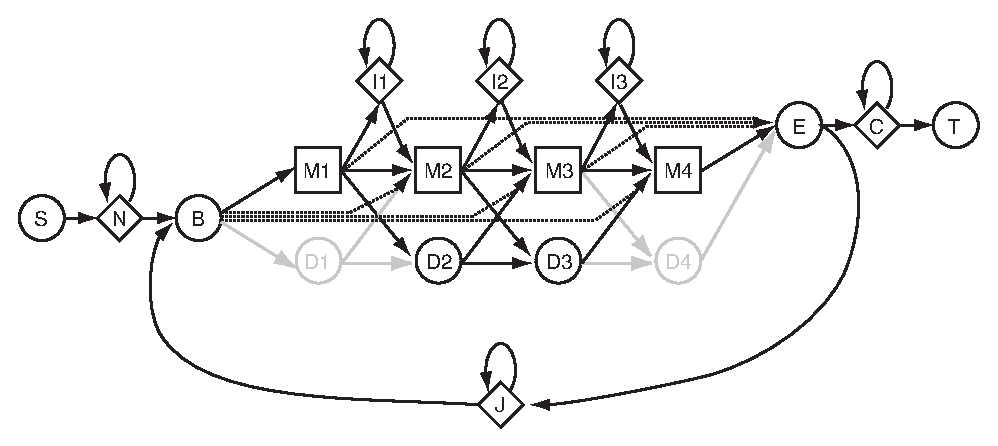
\epsfig{file=plan7.eps}
\caption{\textit{The Plan7 architecture. Squares indicate match states
(modeling consensus positions in the alignment). Diamonds indicate
insert states (modeling insertions relative to consensus) and special
random sequence emitting states. Circles indicate delete states
(modeling deletions relative to consensus) and special begin/end
states. Arrows indicate state transitions. See text for more details.}}
\end{figure}

The section of the model composed of M, D, and I states, and the B and
E states, is essentially a Krogh/Haussler profile HMM. I refer to this
as the ``main model''. A group of three states M/D/I at the same
consensus position in the alignment is called a ``node''. The main
model controls the \textit{data dependent} features of the model.  The
probability parameters in the main model are generally learned from
data in a multiple sequence/structure alignment.

Unlike the original Krogh/Haussler and HMMER model architecture, Plan
7 has no D $\rightarrow$ I or I $\rightarrow$ D transitions. This
reduction from 9 to 7 transitions per node in the main model is the
origin of the codename Plan 7. (The original HMMER architecture is
called Plan 9 in parts of the code.)

The other states (S,N,C,T,J) are called ``special states''. They
(combined with special entry probabilities from B and exit
probabilities to E) control the \textit{algorithm dependent} features
of the model: how likely the model is to generate various sorts of
local or multihit alignments. The algorithm dependent parameters are
typically not learned from data, but rather set externally by choosing
a desired alignment style.

\subsection{Local alignments in Plan 7}

The Plan 7 architecture models a complete sequence, regardless of how
much of that sequence matches the main model. \textit{All alignments
to a Plan 7 model are ``global'' alignments}, but some of the sequence
may be assigned to Plan 7 states (N,C,J) that generate ``random''
sequence that is not aligned to the main model.  Thus, the algorithm
dependent parts of the model control the \textit{apparent} locality of
the alignments.

Local alignments with respect to the sequence (i.e., allowing a match
to the main model anywhere internal to a longer sequence) are
controlled by the N and C states. If the N $\rightarrow$ N transition
is set to 0, alignments are constrained to start in the main model at
the very first residue. Similarly, if the C $\rightarrow$ C transition
is set to 0, alignments are constrained to match the main model at the
very last residue in the sequence.

Local alignments with respect to the model (i.e., allowing fragments
of the model to match the sequence) are controlled by B $\rightarrow$
M ``entry'' transitions and M $\rightarrow$ E ``exit'' transitions,
shown as dotted lines in the Plan 7 figure. Setting all entries but
the B $\rightarrow$ M$_1$ transition to 0 forces a partially
``global'' alignment in which all alignments to the main model must
start at the first match or delete state. Setting all exits to 0 but
the final M $\rightarrow$ E transition (which is always 1.0) forces a
partially global alignment in which all alignments to the main model
must end at the final match or delete state.

Multiple hit alignments are controlled by the E $\rightarrow$ J
transition and the J state. If the E $\rightarrow$ J transition is set
to 0, a sequence may only contain one domain (one alignment to the
main model). If it is nonzero, more than one domain per sequence can
be aligned to the main model. The J $\rightarrow$ J transition
controls the expected length of the intervening sequence between
domains; the lower this probability, the more clustered the domains
are expected to be.

The original HMMER1 search programs are encoded in Plan 7 models as
follows:

\begin{wideitem}
\item [\emprog{hmms}] Simple global alignment. $t_{NN}$ and $t_{CC}$ set to
$t_{GG}$ from the null model (see below). $t_{EJ}$ set to
zero. Internal entries and exits set to zero.

\item [\emprog{hmmls}] Akin to ``profile'' alignment (as Waterman and others
call it): global with respect to main model, local with respect to
sequence, multiple nonoverlapping domains allowed. $t_{NN}$ and
$t_{CC}$ set to $t_{GG}$ from the null model. $t_{EJ}$ set to
0.5. Internal entries and exits set to zero.
 
\item [\emprog{hmmsw}] Smith/Waterman alignment: fully local with 
respect to both the main model and the sequence; single domain.
$t_{NN}$ and $t_{CC}$ set to $t_{GG}$ from the null model. $t_{EJ}$
set to zero. Internal entries are set to $0.5/(M-1)$ for a model with
$M$ match states. Exit probabilities are set such that the overall
chance of exiting from an internal match state is 0.5, and the
posterior probability distribution over which match state is exited is
equal (I'm trying to word this carefully; the M $\rightarrow$ E
probabilities are not equal, because there's a small compensation for
the fact that if you can leave from $M_5$, then the chance that you'll
even get to $M_6$ is reduced.)

\item [\emprog{hmmfs}] Multihit Smith/Waterman alignment. Same
as the above, but $t_{EJ}$ is set to 0.5.
\end{wideitem}


One advantage of Plan 7 is great flexibility in choosing an alignment
style. Complicated alignment styles are easily encoded in the model
parameters without changing the alignment algorithm.  For example, say
you wanted to model human L1 retrotransposon elements. Because of the
way L1 elements are inserted by reverse transcriptase (RVT), L1
elements tend to have a defined 3' end (RVT starts replication at the
same place in each new L1) but a ragged 5' end (RVT prematurely falls
off a new L1 in an unpredictable fashion). A specialized L1 model
could define non-zero internal entry probabilities and zero internal
exit probabilities to model this biological situation.

One disadvantage of Plan 7 is that if you decide you want to do both
local and global alignments, you need two different models (or you
need to do one search, then change the model). This wouldn't be a
terrible burden except for the fact that the algorithm-dependent
parameters strongly affect the values of the $\mu$ and $\lambda$
parameters that E-value statistics depend on. If the algorithm
dependent parameters are changed, these parameters are lost and the
model should be recalibrated with \prog{hmmcalibrate} -- and
\prog{hmmcalibrate} is relatively slow.


\subsection{The Plan 7 null model}

When HMM alignments are scored, they are scored by a log-odds score
relative to a ``null model'' of random sequence composition
\cite{Barrett97}. In Plan 7, this model is now specified as a full
probabilistic model too:

\begin{center}
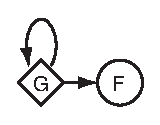
\epsfig{file=nullmodel.eps}
\end{center}

The G state has a symbol emission probability distribution for $K$
symbols in the alphabet. By default, this distribution is set either
to the average amino acid composition of SWISSPROT 34, or to 0.25 for
each nucleotide. The G $\rightarrow$ G transition controls the
expected length of observed random sequences; in practice, this
transition probability is so close to 1 that it has very little
effect. The F state is just a dummy end state like the T state in the
Plan 7 architecture.

\subsection{Wing retraction in Plan 7 dynamic programming}

In the figure of the Plan 7 architecture, you may have noticed that
the first and last delete states are greyed out. Internally in HMMER,
these delete states exist in the ``probability form'' of the model
(when the model is being worked with in every way except alignments)
but they are carefully removed in the ``search form'' of the model
(when the model is converted to log-odds scores and used for
alignments). This process is called ``wing retraction'' in the code,
by analogy to a swept-wing fighter changing from a wings-out takeoff
and landing configuration to a wings-back configuration for high speed
flight.

The problem is that the Plan 7 model allows cycles through the J
state. If a continuous nonemitting ``mute cycle'' were possible (J, B,
D states, E, and back to J), dynamic programming recursions would
fail. This is why special mute states like delete states must be
handled carefully in HMM dynamic programming algorithms; see
\cite{Durbin98} for further discussion. The easiest way to
prevent a mute cycle is to make sure that the model must pass through
at least one match state per path through the main model.

Wing retraction involves folding the probabilities of the terminal
delete paths into the Plan 7 entry and exit probabilities. For
example, in wing retraction the ``algorithm dependent'' B
$\rightarrow$ M$_{3}$ entry probability is incremented by the
probability of the ``data dependent'' path B $\rightarrow$ D$_1$
$\rightarrow$ D$_2$ $\rightarrow$ M$_3$.

Having the wing retraction step, rather than {\em always} folding
these probabilities together, is a design decision, preserving a
distinction between the ``algorithm dependent'' and ``data dependent''
parts of the model.

\section{Sequence file formats}

For all the programs, unaligned sequence files can be in FASTA,
Genbank, EMBL, or SWISS-PROT format, as well as a few other common
file formats. The programs automatically detect what format the file
is in and whether the sequences are DNA, RNA, or protein.

Aligned sequence files can be in ClustalW, GCG MSF, or SELEX
format. SELEX format is a simple format of one line per sequence,
containing the name first, followed by the aligned sequence. ClustalW,
MSF and SELEX alignment files can also be used where unaligned format
files are required; the sequences will be read in and their gaps
removed. 

Full specifications of these file formats and the other formats
recognized by the HMM package are in the file formats chapter near the
end of the guide.

The programs work on RNA, DNA, and protein sequence. They
automatically detect what your sequences are. The behavior of the
programs when a nucleic acid model is used to analyze protein
sequences, or vice versa, is undefined. Certain other situations may
arise (trying to search the ``complementary strand'' of a protein
database, for example) that are nonsensical in certain contexts. Be
forewarned. If you're lucky, the software will issue a snide warning
to you if you try to do something nonsensical, but usually it will
assume you know what you're doing.

\section{Command line options}

If you forget the command-line syntax or available options of any of
the programs, you can type the name of the program with no other
arguments and get a short help message, including summaries of the
common options.

Commonly used options are generally small letters, like \prog{-a}.
More infrequently used options are generally large letters, like
\prog{-A}. Expert or experimental options are generally in the GNU long form,
like \prog{--null2}.

If you call any program with an option {\tt -h}, you get an augmented
help message, including version info (the software version number is
helpful if you report bugs or other problems to me) and a complete
summary of all the available options, including rarely used and
expert/experimental ones.

\section {Environment variables}

HMMER is built to coexist peacefully with the BLAST suite of database
search programs \cite{Altschul91}. HMMER reads the following
environment variables (the examples given use UNIX csh syntax):

\begin{wideitem}
\item [\emprog{BLASTDB}] Location of sequence databases that
	\prog{hmmsearch} will look in, in addition to the current
	working directory.
	Multiple directories are allowed, separated by colons. A
	trailing slash on each path is important to BLAST, but not to HMMER.\\
	Examples: \\
	\user{setenv BLASTDB /nfs/databases/}
        \user{setenv BLASTDB /nfs/databases/:/nfs/moredatabases/}

\item [\emprog{BLASTMAT}] Location of substitution matrices that
	\prog{hmmbuild --pam} (the PAM prior option) can read.
	Although HMMER can parse a colon-separated list, BLAST must
	have a single directory path here.
	Example:\\
	\user{setenv BLASTMAT /nfs/databases/matrix/}

\item [\emprog{HMMERDB}] Location of HMMs, PFAM, or other HMMER
	specific data files. Any program that reads an HMM file
	looks in both HMMERDB and the current working directory.
	Multiple directories are allowed, colon-separated.
	Examples:\\
	\user{setenv HMMERDB /usr/local/lib/hmmer/}
	\user{setenv HMMERDB /usr/local/lib/hmmer/:/nfs/databases/pfam/}
\end{wideitem}

\section{Other profile HMM implementations}

Several implementations of profile HMM methods and related PSSM
methods are available.  Some are listed in the table below.

\begin{center}
\begin{tabular}{ll}
Software  &   URL \\ \hline
HMMER     & \htmladdnormallink{http://hmmer.wustl.edu/}{http://hmmer.wustl.edu/}  \\
SAM       & \htmladdnormallink{http://www.cse.ucsc.edu/research/compbio/sam.html}{http://www.cse.ucsc.edu/research/compbio/sam.html} \\
PFTOOLS   & \htmladdnormallink{http://ulrec3.unil.ch:80/profile/}{http://ulrec3.unil.ch:80/profile/}  \\
HMMpro    & \htmladdnormallink{http://www.netid.com/html/hmmpro.html}{http://www.netid.com/html/hmmpro.html}\\
GENEWISE  & \htmladdnormallink{http://www.sanger.ac.uk/Software/Wise2/}{http://www.sanger.ac.uk/Software/Wise2/} \\
PROBE     & \htmladdnormallink{ftp://ncbi.nlm.nih.gov/pub/neuwald/probe1.0/}{ftp://ncbi.nlm.nih.gov/pub/neuwald/probe1.0/} \\
META-MEME & \htmladdnormallink{http://www.cse.ucsd.edu/users/bgrundy/metameme.1.0.html}{http://www.cse.ucsd.edu/users/bgrundy/metameme.1.0.html} \\
BLOCKS    & \htmladdnormallink{http://www.blocks.fhcrc.org/}{http://www.blocks.fhcrc.org/} \\
PSI-BLAST & \htmladdnormallink{http://www.ncbi.nlm.nih.gov/BLAST/newblast.html}{http://www.ncbi.nlm.nih.gov/BLAST/newblast.html} \\
\end{tabular}
\end{center}

HMMER, SAM, PFTOOLS, and HMMpro are the most closely related to the
profile HMM methods introduced by Krogh et al. HMMpro is commercial,
not free software.
